% interactcadsample.tex
% v1.03 - April 2017

\documentclass[]{interact}

\usepackage{epstopdf}% To incorporate .eps illustrations using PDFLaTeX, etc.
\usepackage{subfigure}% Support for small, `sub' figures and tables
%\usepackage[nolists,tablesfirst]{endfloat}% To `separate' figures and tables from text if required

\usepackage{natbib}% Citation support using natbib.sty
\bibpunct[, ]{(}{)}{;}{a}{}{,}% Citation support using natbib.sty
\renewcommand\bibfont{\fontsize{10}{12}\selectfont}% Bibliography support using natbib.sty

\theoremstyle{plain}% Theorem-like structures provided by amsthm.sty
\newtheorem{theorem}{Theorem}[section]
\newtheorem{lemma}[theorem]{Lemma}
\newtheorem{corollary}[theorem]{Corollary}
\newtheorem{proposition}[theorem]{Proposition}

\theoremstyle{definition}
\newtheorem{definition}[theorem]{Definition}
\newtheorem{example}[theorem]{Example}

\theoremstyle{remark}
\newtheorem{remark}{Remark}
\newtheorem{notation}{Notation}


% tightlist command for lists without linebreak
\providecommand{\tightlist}{%
  \setlength{\itemsep}{0pt}\setlength{\parskip}{0pt}}



\usepackage{lscape}
\usepackage{hyperref}
\usepackage[utf8]{inputenc}
\def\tightlist{}
\usepackage{setspace}
\doublespacing


\begin{document}


\articletype{ARTICLE TEMPLATE}

\title{Automated reading of residual plots with computer vision models}


\author{\name{Weihao Li$^{a}$}
\affil{$^{a}$Department of Econometrics and Business Statistics, Monash
University, Clayton, VIC, Australia}
}

\thanks{CONTACT Weihao
Li. Email: \href{mailto:weihao.li@monash.edu}{\nolinkurl{weihao.li@monash.edu}}}

\maketitle

\begin{abstract}
TBD.
\end{abstract}

\begin{keywords}
TBD
\end{keywords}

\hypertarget{introduction}{%
\section{Introduction}\label{introduction}}

The practice of plotting residuals is commonly regarded as a standard
procedure in linear regression diagnostics
\citep[see][]{cook1982residuals, belsley1980regression}. This visual
assessment plays a crucial role in identifying deviations from model
assumptions, such as linearity, homoscedasticity, and normality. It also
helps in understanding the goodness of fit and various characteristics
of the model.

Generating a residual plot in most statistical software is often as
straightforward as executing a line of code or clicking a button.
However, accurately interpreting a residual plot can be challenging.
Consider Figure \ref{fig:false-finding} as an example, the residuals
display a triangular shape pointing to the left. While this might
suggest heteroskedasticity, it is important to avoid over-interpreting
the visual pattern. In this case, the fitted model is correctly
specified, and the triangular shape is actually a result of the skewed
distribution of the predictors, rather than indicating a flaw in the
model.

A residual plot can exhibit various visual features, but it is crucial
to recognize that some may arise from the characteristics of predictors
and the inherent randomness of the error, rather than indicating a
violation of model assumptions \citep{li2023plot}. The concept of visual
inference, as proposed by \citet{buja2009statistical}, provides an
inferential framework to assess whether residual plots indeed contain
visual patterns inconsistent with the model assumptions. The fundamental
idea involves testing whether the actual residual plot visually differs
significantly from null plots, which are created using residuals
generated from the null distribution. Typically, this is accomplished
through the lineup protocol. In this approach, the real residual plot is
embedded within a lineup alongside several null plots. If the real
residual plot can be distinguished from the lineup, it provides evidence
for rejecting the null hypothesis.

The practice of delivering a residual plot as a lineup is generally
regarded as a valuable approach. Beyond its application in residual
diagnostics, the lineup protocol has integrated into the analysis of
diverse subjects. For instance,
\cite{loy2013diagnostic, loy2014hlmdiag, loy2015you} illustrate its
applicability in diagnosing hierarchical linear models. Additionally,
\citet{widen2016graphical} demonstrates its utility in geographical
research, while \citet{krishnan2021hierarchical} explores its
effectiveness in forensic examinations.

However, as pointed out by \citet{li2023plot}, a primary limitation of
the lineup protocol lies in its reliance on human judgments. Unlike
conventional statistical tests that can be performed numerically and
automatically in statistical software, the lineup protocol requires
human evaluation of images. This characteristic makes it less suitable
for large-scale applications, given the associated high labour costs and
time requirements.

There is a substantial need to develop an approach that alleviates
people's workload by automating repetitive tasks and providing
standardized results in a controlled environment. The large-scale
evaluation of lineups is impractical without the use of technology and
machines.

The utilization of computers to interpret data plots has a rich history,
with early efforts such as ``Scagnostics'' by \citet{tukey1985computer},
focusing on scatterplot diagnostics. \citet{wilkinson2005graph} expanded
on this work, introducing graph theoretic scagnostics, which encompassed
nine computable measures applied to planar proximity graphs. These
measures, including ``Outlying'', ``Skinny'', ``Stringy'', ``Straight'',
``Monotonic'', ``Skewed'', ``Clumpy'', and ``Striated'' aimed to
characterize outliers, shape, density, trend, and coherence of the data.
While this approach has been inspiring, there is a recognition
\citep{buja2009statistical} that it may not capture all the necessary
visual features that differentiate actual residual plots from null
plots. A more promising alternative entails enabling computers to learn
the function for extracting visual features from residual plots.
Essentially, this means empowering computers to discern the crucial
visual features for residual diagnostics and determining the method to
extract them. Modern computer vision models are well-suited for
addressing this challenge.

Modern computer vision models often rely on deep neural networks with
convolutional layers \citep{fukushima1982neocognitron}. These layers
leverage hierarchical patterns in data, downsizing and transforming
images by summarizing information in a small space. Numerous studies
have demonstrated the efficacy of convolutional layers in addressing
various vision tasks, including image recognition \citep{rawat2017deep}.
Despite the widespread use of computer vision models in fields like
computer-aided diagnosis \citep{lee2015image}, pedestrian detection
\citep{brunetti2018computer}, and facial recognition
\citep{emami2012facial}, their application in reading data plots remains
limited. While some studies have explored the use of computer vision
models for tasks such as reading recurrence plots for time series
regression \citep{ojeda2020multivariate}, time series classification
\citep{chu2019automatic, hailesilassie2019financial, hatami2018classification, zhang2020encoding},
anomaly detection \citep{chen2020convolutional}, and pairwise causality
analysis \citep{singh2017deep}, the application of reading residual
plots with computer vision models represents a relatively new field of
study.

In this paper, we develop computer vision models and integrate them into
the residual plots diagnostics workflow, filling the gap of\ldots. The
paper is structured as follows: \ldots{}

\begin{figure}

{\centering 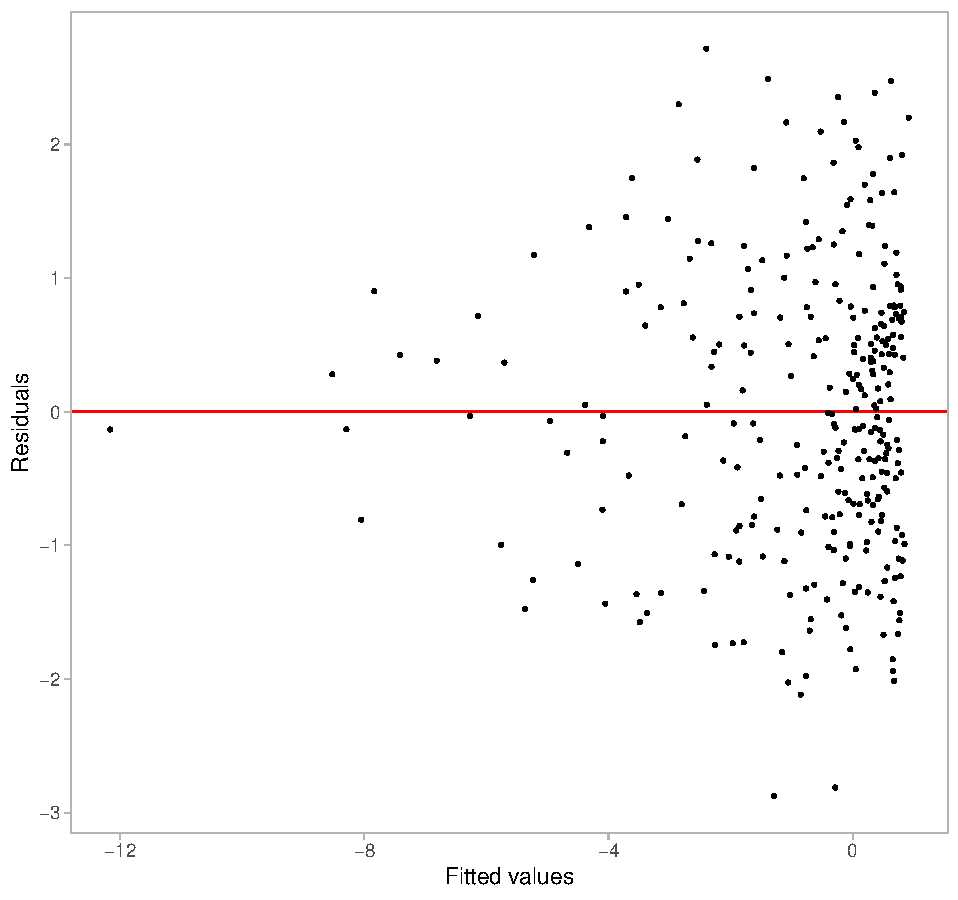
\includegraphics[width=1\linewidth]{paper_files/figure-latex/false-finding-1} 

}

\caption{An example residual vs fitted values plot (red line indicates 0). The vertical spread of the data points varies with the fitted values. This often indicates the existence of heteroskedasticity.}\label{fig:false-finding}
\end{figure}

\hypertarget{methodogology}{%
\section{Methodogology}\label{methodogology}}

\hypertarget{distance-from-the-good-residual-plots}{%
\subsection{Distance from the good residual
plots}\label{distance-from-the-good-residual-plots}}

In a visual test, the observer will be asked to choose one or more plots
that stand out as most distinct from others in a given lineup. To
develop a computer vision model for evaluating residual plots within the
visual inference framework, it is important to precisely define a
numerical measure of ``difference'' or ``distance'' between plots. This
distance can take the form of a basic statistical operation on pixels,
such as the sum of square differences. Alternatively, it could involve
established image similarity metrics like the Structural Similarity
Index Measure (SSIM) (ref here). The challenge lies in the fact that
metrics tailored for image comparison may not be suitable for evaluating
data plots, where only essential plot elements require assessment
\citep{chowdhury2018measuring}.

\hypertarget{residual-distribution}{%
\subsubsection{Residual distribution}\label{residual-distribution}}

The distance metrics proposed in this paper takes into account the fact
that we try to measure how different a residual plot is from a good
residual plot, or in other words, how different a given fitted model is
from a correctly specified model. For classical normal linear regression
model, residuals are derived from the fitted values
\(\hat{\boldsymbol{y}}\) and observed values \(\boldsymbol{y}\).
However, if the data generating process is known and the model is
correctly specified, by the Frisch-Waugh-Lowell theorem (ref here),
residuals \(\boldsymbol{e}\) can be written as a linear transformation
of the error \(\boldsymbol{\varepsilon}\):

\begin{equation}
\label{eq:residual-1}
\boldsymbol{e} = \boldsymbol{R}\boldsymbol{\varepsilon},
\end{equation}

\noindent where
\(\boldsymbol{R}=\boldsymbol{I}_n -\boldsymbol{X}(\boldsymbol{X}'\boldsymbol{X})^{-1}\boldsymbol{X}'\)
is the residual operator, \(\boldsymbol{X}\) is the design matrix,
\(\boldsymbol{I}_n\) is a \(n\) by \(n\) identity matrix, and \(n\) is
the number of observations.

One of the assumptions of the classical normal linear regression model
is the error \(\boldsymbol{\varepsilon}\) follows a multivariate normal
distribution with zero mean and constant variance, i.e.,
\(N(\boldsymbol{0}_n,\sigma^2\boldsymbol{I}_n)\). Using equation
\ref{eq:residual-1}, it can be known that residuals \(\boldsymbol{e}\)
also follow a certain probability distribution, which will be denoted as
\(Q\). This reference distribution \(Q\) summarises what good residuals
should follow given the predictors are known and fixed.

Probability distribution \(Q\) is actually a degenerate multivariate
distribution due to the fact that \(rank(\boldsymbol{R}) = n - 1 < n\).
This means the \(n\)th residual value will be known given the \(n - 1\)
residuals. To capture the exact characteristics of \(Q\), such as
moments, we can simulate a large numbers of \(\boldsymbol{\varepsilon}\)
and transform it to \(\boldsymbol{e}\). For simplicity, we replaced
\(\boldsymbol{R}\) with a diagonal matrix \(diag(\boldsymbol{R})\). The
resulting distribution for \(\boldsymbol{Q}\) is
\(N(\boldsymbol{0}_n, diag(\boldsymbol{R}\sigma^2))\).

If the model is misspecified, then the actual distribution of residuals
denoted as \(P\), will be different to \(Q\). For example, if the model
formula is correct, but the error \(\boldsymbol{\varepsilon}\) follows a
multivariate lognormal distribution, \(P\) will not be the same as \(Q\)
and we would expect a skewed empirical distribution for residuals. And
if there is an omitted variable problem, then the residual operator
obtained from the fitted model will not be the same as
\(\boldsymbol{R}\), and again, \(P\) will be different to \(Q\).

\hypertarget{kullback-leibler-divergence-of-p-from-q}{%
\subsubsection{\texorpdfstring{Kullback-Leibler divergence of \(P\) from
\(Q\)}{Kullback-Leibler divergence of P from Q}}\label{kullback-leibler-divergence-of-p-from-q}}

Define a proper distance between distributions is usually easier than
define a proper distance between data plots. Given the actual residual
distribution \(Q\) and the reference residual distribution \(P\), we
used a distance metric based on Kullback-Leibler divergence (ref here)
to quantify the difference between two distributions

\begin{align}
D &= log\left(1 + KL\right), \\
\label{eq:kl-1}
KL &= \int_{\mathbb{R}^{n}}log\frac{p(\boldsymbol{e})}{q(\boldsymbol{e})}p(\boldsymbol{e})d\boldsymbol{e},
\end{align}

\noindent where \(p(\boldsymbol{e})\) is the probability density
function for distribution \(P\), and \(q(\boldsymbol{e})\) is the
probability density function for distribution \(Q\).

This distance metric was first proposed in \citet{li2023plot}. It was
mainly designed for measuring the effect size of non-linearity and
heteroskedasticity in a residual plot. For a linear regression model
that has omitted higher-order predictors \(\boldsymbol{Z}\) along with
coefficients \(\boldsymbol{\beta}_z\), and an error distribution
\(N(\boldsymbol{0}_n, \boldsymbol{V})\), \(Q\) can be represented as
\(N(\boldsymbol{R}\boldsymbol{Z}\boldsymbol{\beta}_z, diag(\boldsymbol{R}\boldsymbol{V}\boldsymbol{R}'))\).
Note that the variance-covariance matrix is replaced with its diagonal
analogy to ensure it is a full rank matrix.

Since both \(P\) and \(Q\) are adjusted to be multivariate normal
distributions, equation \ref{eq:kl-1} can be further expanded to

\begin{align}
\label{eq:kl-2}
KL &= \frac{1}{2}\left(\log\frac{|\text{diag}(\boldsymbol{W})|}{|\text{diag}(\boldsymbol{R}\sigma^2)|} - n + \text{tr}(\text{diag}(\boldsymbol{W})^{-1}\text{diag}(\boldsymbol{R}\sigma^2)) + \boldsymbol{\mu}_z'(diag(\boldsymbol{W}))^{-1}\boldsymbol{\mu}_z\right),
\end{align}

\noindent where
\(\boldsymbol{\mu}_z = \boldsymbol{R}\boldsymbol{Z}\boldsymbol{\beta}_z\),
and \(\boldsymbol{W} = \boldsymbol{R}\boldsymbol{V}\boldsymbol{R}'\).
The assumed error variance \(\sigma^2\) is set to be
\(tr(\boldsymbol{V})/n\), which is the expectation of the estimated
variance.

\hypertarget{evaluation-of-kullback-leibler-divergence-for-non-normal-p}{%
\subsubsection{\texorpdfstring{Evaluation of Kullback-Leibler divergence
for non-normal
\(P\)}{Evaluation of Kullback-Leibler divergence for non-normal P}}\label{evaluation-of-kullback-leibler-divergence-for-non-normal-p}}

For non-normal error \(\boldsymbol{\varepsilon}\), the actual residual
distribution \(P\) is unlikely to be a multivariate normal distribution.
Thus, equation \ref{eq:kl-2} will not be applicable to linear regression
model with non-normality issue.

To evaluate the Kullback-Leibler divergence of non-normal \(P\) from
\(Q\), we need to solve equation \ref{eq:kl-1}. However, since
\(\boldsymbol{e}\) is a linear transformation of non-normal random
variables, it is very common that the general form of \(P\) is unknown,
meaning that we can not easily compute \(p(\boldsymbol{e})\) using a
well-known probability density function.

Additionally, even if \(p(\boldsymbol{e})\) can be calculated for any
\(\boldsymbol{e} \in \mathbb{R}^n\), it will be very difficult to do
numerical integration over the \(n\) dimensional space, because \(n\)
could be potentially very large.

In order to evaluate equation \ref{eq:kl-1} in a practically computable
manner, the elements of \(\boldsymbol{e}\) are assumed to be independent
of each other. This assumption solves both of the issues mentioned
above. First, we no longer need to integrate over \(n\) random
variables. The result is now the sum of the Kullback-Leibler divergence
evaluated for each individual residual thanks for the independence
assumption. Second, it is not required to know the joint probability
density \(p(\boldsymbol{e})\) any more. Instead, the evaluation of
Kullback-Leibler divergence for a single residual relies on the
knowledge of \(p(e_i)\), where \(e_i\) is the \(i\)th residual for
\(i = 1, ..., n\). This is much easier to estimate through simulation.

The algorithm to compute equation \ref{eq:kl-1} starts from simulating
\(m\) sets of \(\boldsymbol{\varepsilon}\) according to the error
distribution. The simulated errors are stored in a matrix
\(\boldsymbol{A}\) with \(n\) rows and \(m\) columns. So each column of
\(\boldsymbol{A}\) is a set of realization values of
\(\boldsymbol{\varepsilon}\). Then, we can get \(m\) sets of
\(\boldsymbol{e}\) stored in the matrix \(\boldsymbol{B}\) by applying
the residual rotation operator
\(\boldsymbol{B} = \boldsymbol{R}\boldsymbol{A}\). Furthermore, kernel
density estimation (ref here) is applied on each row of \(B\) to
estimate \(p(e_i)\) for \(i = 1, ..., n\).

Since the Kullback-Leibler divergence can be viewed as the expectation
of the log-likelihood ratio between distribution \(P\) and distribution
\(Q\) evaluated on distribution \(P\), we can reuse the simulated
residuals in matrix \(\boldsymbol{B}\) to compute the expectation.
Therefore, the Kullback-Leibler divergence can be formulated as

\begin{align}
\label{eq:kl-3}
KL &= \sum_{i = 1}^{n} KL_i, \\
KL_i &= \frac{1}{m}\sum_{j = 1}^{m} log\frac{p(B_{ij})}{q(B_{ij})},
\end{align}

\noindent where \(KL_i\) is the Kullback-Leibler divergence for an
individual residual \(e_i\), \(B_{ij}\) is the \(i\)th row and \(j\)th
column entry of the matrix \(B\), \(q(.)\) is the normal density
function with mean zero and an assumed variance estimated as
\(\hat{\sigma^2} = var(flatten(B))\), and \(flatten(.)\) unfolds a
matrix into a vector.

\hypertarget{approximation-of-the-distance-metric-with-a-residual-plot}{%
\subsubsection{Approximation of the distance metric with a residual
plot}\label{approximation-of-the-distance-metric-with-a-residual-plot}}

In the previous sections, we have defined a distance metric for
quantifying the difference between the actual residual distribution and
an ideal reference distribution. This distance metric can only be
computed when the data generating process is known. In reality, we often
have no knowledge about the data generating process, otherwise we do not
need to fit a linear regression model in the first place.

What we proposed in this paper is a method to approximate this distance
with a residual plot. This is done by training computer vision models
with a large number of pairs of residual plots and distance. With the
approximated distance, we will be able to know how different the
underlying distribution of the residuals is from a good residual
distribution. This is meaningful way to check if a residual plot is a
good residual plot, and to know the strength of the visual signal
indicating model violations.

The approximated distance is not expected to be the same as the original
distance. This is largely because information embedded in a single
residual plot is limited and it may not be able to summarise the
characteristics of the residual distribution. For a given residual
distribution \(P\), we can generate many different residual plots. Some
of them share similar visual patterns, but some of them could be
visually very different from the rest, especially for models with small
\(n\). This suggests the approximated distance will vary depends on
whether the observed residual plot is representative or not.

\hypertarget{generation-of-simulated-training-data}{%
\subsection{Generation of simulated training
data}\label{generation-of-simulated-training-data}}

The computer vision models we developed in this study were trained with
synthetic data. This means the training data and the test data were
simulated from a known data generating process under different parameter
settings.

We have incorporated three types of residual departures of linear
regression model in this study, including non-linearity,
heteroskedasticity and non-normality.

\begin{align*}
\boldsymbol{y} &= \boldsymbol{1}_n + \boldsymbol{x}_1 + \beta_1\boldsymbol{x}_2 + \beta_2(\boldsymbol{z} + \beta_1\boldsymbol{w}) + \boldsymbol{k} \odot \boldsymbol{\varepsilon}, \\
\boldsymbol{z} &= He_j(g(\boldsymbol{x}_1, 2)), \\
\boldsymbol{w} &= He_j(g(\boldsymbol{x}_2, 2)), \\
\boldsymbol{k} &= \sqrt{\boldsymbol{1}_n + b(2 - |a|)(\boldsymbol{x}_1 + \beta_1\boldsymbol{x}_2 - a\boldsymbol{1}_n)^2}, \\
\boldsymbol{\varepsilon} &\sim N(\boldsymbol{0}_n, \boldsymbol{I}_n),
\end{align*}

\noindent where \(\boldsymbol{y}\), \(\boldsymbol{x}_1\),
\(\boldsymbol{x}_2\), \(\boldsymbol{z}\), \(\boldsymbol{w}\),
\(\boldsymbol{k}\) and \(\boldsymbol{\varepsilon}\) are vectors of size
\(n\), \(\boldsymbol{1}_n\) is a vector of ones of size \(n\),
\(He_j(.)\) is the \(j\)th-order probabilist's Hermite polynomials
(ref), the \(\sqrt{(.)}\) and \((.)^2\) operator are element-wise
operators, \(\odot\) is the Hadamard product, and \(g(., k)\) is a
scaling function to enforce the support of the random vector to be
\([-k, k]^n\) defined as

\[g(\boldsymbol{x}, k) = 2k \cdot \frac{\boldsymbol{x} - x_{min}\boldsymbol{1}_n}{x_{max} - x_{min}} - k\boldsymbol{1}_n,~for~k > 0,\]
\noindent where \(x_{min} = \underset{i \in \{ 1,...,n\}}{min} x_i\),
\(x_{max} = \underset{i \in \{ 1,...,n\}}{max} x_i\) and \(x_i\) is the
\(i\)-th entry of \(\boldsymbol{x}\).

\hypertarget{different-configurations-of-the-model-formula}{%
\subsection{Different configurations of the model
formula}\label{different-configurations-of-the-model-formula}}

discuss different types of inputs and output choices, and why we choose
the current design

\hypertarget{architecture-of-the-computer-vision-model}{%
\subsection{Architecture of the computer vision
model}\label{architecture-of-the-computer-vision-model}}

\hypertarget{training-process-and-hyperparameter-tuning}{%
\subsection{Training process and hyperparameter
tuning}\label{training-process-and-hyperparameter-tuning}}

\hypertarget{model-evaluation-methods}{%
\subsection{Model evaluation methods}\label{model-evaluation-methods}}

\hypertarget{results}{%
\section{Results}\label{results}}

\hypertarget{best-model-performance}{%
\subsection{Best model performance}\label{best-model-performance}}

\begin{itemize}
\tightlist
\item
  Metrics for model performance
\item
  Shap values
\item
  Heatmap
\end{itemize}

\hypertarget{comparison-with-human-visual-inference}{%
\subsection{Comparison with human visual
inference}\label{comparison-with-human-visual-inference}}

\hypertarget{overview-of-the-human-subject-experiment}{%
\subsubsection{Overview of the human subject
experiment}\label{overview-of-the-human-subject-experiment}}

\hypertarget{comparison}{%
\subsubsection{Comparison}\label{comparison}}

\begin{itemize}
\tightlist
\item
  power comparison
\item
  decisions
\end{itemize}

\hypertarget{when-the-model-works}{%
\subsection{When the model works}\label{when-the-model-works}}

\begin{itemize}
\tightlist
\item
  simple examples (non-linearity, heteroskedasticity, \ldots)
\item
  datasaurus
\end{itemize}

\hypertarget{when-the-model-does-not-work}{%
\subsection{When the model does not
work}\label{when-the-model-does-not-work}}

\begin{itemize}
\tightlist
\item
  human detect but model does not
\item
  cartoon residuals?
\end{itemize}

\hypertarget{workflow-how-one-use-this-model-small-showcase}{%
\subsection{Workflow: how one use this model? (small
showcase)}\label{workflow-how-one-use-this-model-small-showcase}}

\hypertarget{dicussion}{%
\section{Dicussion}\label{dicussion}}

\hypertarget{conclusion}{%
\section{Conclusion}\label{conclusion}}

\begin{itemize}
\tightlist
\item
  Summary of findings
\item
  Contributions to the field
\item
  Future directions for research
\end{itemize}

\bibliographystyle{tfcad}
\bibliography{ref.bib}





\end{document}
